\documentclass[12pt]{article}
\usepackage[utf8]{inputenc}
\usepackage{color}
\usepackage{polski}
\usepackage{graphicx}
\usepackage{pdfpages}
\usepackage{indentfirst}
\usepackage{geometry}
\usepackage{setspace}
\usepackage[hyphens]{url}
\usepackage[style=numeric, backend=biber]{biblatex}
\usepackage{array}
\usepackage{float}

\addbibresource{bibliography.bib}
\graphicspath{{./images/}}

\setstretch{1.5}

\geometry{
  a4paper,
  left=30mm,
  top=25mm,
  right=10mm,
  bottom=20mm
}

\begin{document}
\begin{sloppypar}

\includepdf{strona_tytulowa.pdf}

\tableofcontents
\newpage

\section{Wprowadzenie}
{
  W dobie trwającego rozwoju technologicznego, każdy aspekt życia codziennego jest usprawniany i przenoszony
  do internetu. Nieinaczej jest z promowaniem i sprzedażą biletów na wydarzenie kulturowe pokroju:
  spektakli w teatrze, koncertów, festiwali. Aplikacja ConcertsApp ma służyć dokładnie temu,
  ma zminimalizować czas, jaki należałoby kiedyś przeznaczyć na zdobycie biletów. Czy też na uzyskanie
  informacji o wydarzeniach z interesującej konsumenta dziedziny, lub odbywającę się w pobliżu.
  \subsection{Problematyka}
  {
    ?????????????????????????????????????????????????????????????????
  }
  \subsection{Cel i założenia pracy}
  {
    Celem niniejszej pracy dyplomowej jest stworzenie aplikacji webowej, która umożliwi w łatwy i szybki
    sposób na promowanie wydarzeń kulturowych i zakup biletów na nie. Zakup odbywać się będzie za pomocą
    płatności online, jedynie podając dane karty kredytowej lub debetowej, lub poprzez stworzenie konta.\par
    Zakres pracy obejmuję zaprojektowanie i implementację aplikacji klienckiej i serwerowej, przy
    wykorzystaniu, najnowszych i bardzo popularnych na rynku pracy, technologii. Do strony klienckiej
    został wykorzystany React, z koleji do stworzenia serwera użyto Node.JS.
  }
  \subsection{Struktura pracy inżynierskiej}
  {
    Pierwszy rozdział ma posłużyć jako wprowadzenie do problemu podjętego w niniejszej pracy dyplomowej.
    Następny przedstawia aspekty takie jak: konkurencyjne rozwiązania do tworzonej aplikacji,
    analiza najpopularniejszych metod płatności online, opowiada o bazach danych oraz przybliża
    metody tworzenie aplikacji webowych.
    Trzeci rozdział przedstawia wykorzystane technologie do implementacji aplikacji oraz uzasadnia dlaczego
    akurat ona została wybrana a nie inna.
    Czwarty rozdział pokazuje jak przebiegał proces twórczy, czyli projektowanie i implementacja.
  }
}

\section{Teoria niezbędna do realizacji projektu}
{
  \subsection{Analiza istniejących portali do promowania i dystrybucji biletów na wydarzenia kulturowe}
  {
    Najpopularniejszymi portalami zbliżonymi do tworzonej aplikacji są zdecydowanie:
    \begin{itemize}
      \item Eventim
      \item GoingApp
    \end{itemize}
    Eventim jest znacznie starszym portalem, co można stwierdzić chociażby, po jego szacie graficznej,
    łatwo to zauważyć porównująć do wyżej wymienionego GoingApp. 
    W swojej ofercie ma wydarzenia pokroju: koncertów, przedstawień teatralnych, oper czy baletów.\\
    Same bilety sprzedawane są w formie papierowej, przychodzą na maila, 
    lub istnieje możliwość zakupu biletu mobilnego. Kupno może odbyć się zarówno poprzez strone internetową, 
    jak również poprzez aplikację mobilną. Płatności można dokonać za pomocą przelewu tradycyjnego, karty kredytowej, szybkiego przelewu Dotpay\\
    GoingApp charakteryzuje się bardziej nowoczesną i przejrzystą szatą graficzną w porównaniu do Eventim. 
    Oferty obu portali są bardzo do siebie zbliżone, lecz tutaj można znaleźć takie wydarzenia, jak chociażby imprezy związane z filmem czy jedzeniem.
    Jednakże nie posiada on biletów na balet lub opery.\\
    Wejściówki można, podobnie jak w Eventim nabyć poprzez ich stronę internetową lub aplikację mobilną. 
    Sam bilet jest dostępny w formie dokumentu PDF, lub kodu QR, dostęp do niego mamy zarówno poprzez maila,którego otrzymujemy zaraz po zakupie, oraz aplikację.
    Użytkownik może dokonać płatności za pomocą systemów płatniczych takich jak: payU, eCard, MasterPass oraz Paymento\textregistered \\
    Aplikacja webowa tworzona na potrzeby niniejszej pracy inżynierskiej czerpie z obu portali najlepsze cechy. 
    Z Eventim czerpie różnorodność wydarzeń, z koleji z GoingApp przejrzystość interfejsu i bilety w formie, bardzo popularnego kodu QR.
    Metody płatności zostają ograniczone do kart płatniczych: debetowej i kredytowej. Podawane są numer karty, data ważności oraz kod CVV.
  }
  \subsection{Zakupy internetowe}
  {
    Sklepy internetowe z roku na rok rosną w siłę, przybywa ich liczba w zatrważającym tempie. 
    Aż 73\% ankietowanych w raporcie przygotowanym przez Gemius Polska\cite{gemius-report} deklaruje kupowanie online i ta forma zakupów cieszy się niezmiennie dobrym 
    wizerunkiem wśród kupujących. Brak sklepu internetowego stanowi ogromną niekorzyść dla obecnych przedsiębiorców. 
    Zakupy online charakteryzują się dużo większym wyborem produktów, łatwością w porównywaniu ofert czy też łatwością w znalezieniu interesujących produktów. 
    Lecz, to nie z wyżej wymienionych powodów, sklepy w sieci cieszą sie taką popularnością.
    Wśród najczęściej wymienianych powodów są: dostępność przez całą dobę (aż 82\% wybrało ten powód), brak konieczności wyjazdu do sklepu - 78\%, 
    nieograniczony czas wyboru - 72\% oraz atrakcyjniejsze ceny niż w sklepach tradycyjnych - 71\%.\\
    Niestety taka forma zakupów ma też swoje słabe strony, najpopularniejszymi
    wymienianymi, napotkanymi problemami są: wysokie koszta dostawy, długi czas oczekiwania na dostawę, irytujące reklamy produktów, wcześniej poszukiwanych.
    Również bardzo często wymienianą przeciwnością jest uszkodzona przesyłka w transporcie, wynikać to może ze źle zapakowanej i zabezpieczonej paczkim lub z winy 
    firmy kurierskiej i jej pracowników.\\
    Co jednak sprawia, że klienci decydują się na wybór danego portalu na zakupy?\\
    Najczęściej wybór sklepu pada dzięki kodom rabatowym, dopiero w dalszej kolejności padają hasła takie jak dokładne informacje o warunkach zamówienia,
    dostępne na stronie dane firmy czy przejrzysta i funkcjonalna strona internetowa. Wydawać by się mogło, że to na te kolejne cechy portali, powinno się w pierwszej kolejności
    zwracać uwagę, bo to dzięki nim w pierwszej chwili można stwierdzić czy strona jest fałszywa, czy też nie.
  }
  \subsection{Analiza najpopularniejszych internetowych metod płatności online} % strona 119 raportu, strona 80 wstep, strona 89 czynniki motywujace do robienia zakupow online
  {
    Najpopularniejszymi metodami płatności w internecie, według raportu "E-commerce w Polsce 2020"\cite{gemius-report} są kolejno:
    \begin{itemize}
      \item szybki przelew przez serwis płatności np. payU, przelewy24
      \item przelew tradycyjny
      \item płatność kartą płatniczą przy składaniu zamówienia
      \item płatności mobilne np. BLIK
    \end{itemize}
    Nie zostały wymienione płatności pokroju wysyłki za pobraniem, płatności w sklepie przy odbiorze, ponieważ nie są to płatności realizowane online, 
    a tych dotyczy analiza przedstawiona w niniejszym rozdziale.\\
    Zdecydowanie nie powinna dziwić obecność szybkich przelewów na pierwszym miejscu tego rankingu. Aż 70\% ankietowanych odpowiedziało, 
    że choć raz korzystało z tej metody, przy robieniu zakupów przez internet. Cechują się błyskawiczynym czasem realizacji, w przeciwieństwie do tradycyjnych
    przelewów. Zaledwie 46\% ankietowanych zdecydowało się choć raz na przelew tradycyjny. Różnica jest znaczna, jednakże nie powinna ona dziwić, ponieważ 
    to oszczędność czasu, poniekąd sprawia, że klienci decydują się na zakupy online w pierwszej kolejności. Przelewy tradycyjne dodatkowo wydłużają czas realizacji 
    zamówienia, ponieważ ich przetwarzanie odbywa się jedynie w dni robocze, o wyznaczonych godzinach, różnych, w zależności od banku.\\
    Na płatność kartą decyduje się 40\% zapytanych, jest to dość zaskakujące, zważywszy na fakt, że jest to zdecydowanie jedna z najszybszych metod płatności. 
    Do jej realizacji niezbędne jest jedynie numer karty, data wygaśnięcia oraz kod CVV. Powodem na dość niską popularność tej metody, mogą być dwie rzeczy, 
    strach przed podawaniem danych karty, żeby nie zostały skradzione. Inną alternatywą czemu, tak mało klientów sklepów internetowych decyduję się na inne metody, 
    jest brak karty podczas składania zamówienia. Pierwsza z nich wydaję się być bardziej prawdopodobna, mało kto kupując 
    produkty przez internet ma akurat przy sobie kartę płatniczą, by odczytać z niej niezbędne liczby. 
    Zdecydowanie łatwiej jest zalogować się do banku i wykonać przelew czy to tradycyjny czy szybki.\\
    Dziwić może obecność płatności mobilnych na ostatnim miejscu z zaledwie 35\% wykorzystania. Jest to sposób bardzo wygodny, zważywszy na fakt iż mało kto 
    nie posiada przy sobie telefonu. Potrzebna jest jeszcze tylko aplikacja banku i można dokonywać dowolnych płatności. W przypadku BLIK-u generowany jest sześcio 
    cyfrowy ciąg liczb, który wystarczy wpisać w odpowienie pole, zatwierdzić płatność w aplikacji i gotowe.
  }
  \subsection{Bazy danych jako środek przechowywania danych}
  {
    "Baza danych to zorganizowany zbiór ustrukturyzowanych informacji, czyli danych, zwykle przechowywany w systemie komputerowym w formie elektronicznej. 
    Bazą danych steruje zwykle system zarządzania bazami danych (DBMS). 
    Dane i system DBMS oraz powiązane z nimi aplikacje razem tworzą system bazodanowy, często nazywany w skrócie bazą danych.". \cite{oracle-db}
    Innymi słowy jest to kontener na dane, w dowolnej postaci, mogą to być liczby, ciągi znaków, a nawet zdjęcia czy filmy. Dane te nie są, najczęściej, przetrzymywane
    lokalnie na komputerach, tylko na serwerach czy w chmurze. \\
    Dlaczego więc korzysta się z baz danych a nie np. z arkuszy kalkulacyjnych?\\
    Odpowiedź jest bardzo prosta, arkusze kalkulacyjne nie zostały stworzone do pracy z ogromną ilością danych, przy jednoczesnym dostępie, nawet kilkuset lub więcej użytkowników.
    Są wręcz idealne do pracy z mniejszą ilościa danych dla jednego lub małej grupy użytkowników, którzy nie potrzebują wielu skomplikowanych funkcji do manipulacji danymi.
    Bazy danych z koleji, przeznaczone są do pracy z ogromnymi ilościami informacji, umożliwiając dodatkowo jednoczesny dostęp do nich, wielu użytkownikom na raz. 
    Co więcej praca z bazami danych, charakteryzuje się wysokim bezpieczeństwem i szybkością wykonywanych operacji. Operacje na danych, tworzenie zapytań odbywa się 
    za pomocą logiki i języka o wysokim stopniu złożoności. Jako przykład może posłużyć, zdecydowanie najpopularniejszy z nich, czyli język zapytań SQL.\\
    Bazy danych dzielimy, między innymi na:
    \begin{itemize}
      \item relacyjne
      \item hurtownie danych
      \item NoSQL
      \item chmurowe
    \end{itemize}
    Relacyjne bazy danych zyskały ogromną popularność w latach 80\cite{oracle-db}. Dane zorganizowane są w tabelach, składające się z wierszy i kolumn. Po dziś dzień stanowią 
    jedne z najpopularniejszych baz danych, jak nie najpopularniejsze, dostępne na rynku. Przykładami relacyjnych baz danych są: MySQL i Microsoft SQL Server.\\
    Hurtownie danych, inaczej centralne repozytorium danych, to typ bazy danych wykorzystywany do wykonywania zapytań i analizy. 
    Ma on umożliwić i wspierać działania z zakresu analizy biznesowej, w szczególności analityki. Często operuje na danych historycznych, pochadzących z wielu źródeł. 
    Jej umiejętności analityczne pozwalają przedsiębiorstwom cenne dane biznesowe, które ułatwiają podejmowanie decyzji.\cite{oracle-warehouse}\\
    Baza danych NoSQL, inaczej nierelacyjna, cechuje się przechowywaniem danych w nieuporządkowany i częściowo uporządkowanych oraz manipulowanie nimi. Od relacyjnych baz
    różni je przede wszystkim to, że w relacyjnych mają jasną strukturę organizacji danych. W nierelacyjnych dane, pochodzące z tej samej kolekcji, mogą posiadać 
    kompletnie różne atrybuty. Szerzej na temat baz NoSQL zostanie omówione w następnym podrodziale.\\
    Ostatnim typem bardzo popularnym na rynku baz danych są bazy chmurowe. Bazy te charakteryzują się przede wszystkim tym, że dane przetrzymywane są na prywatnej,
    publicznej lub hybrydowej platformie przetwarzania danych w chmurze. 
    Najpopularniejszymi bazami w chmurze są Microsoft Azure SQL Database, Oracle Database, Google Cloud SQL oraz Amazon Relational Database Service.
  }
  \subsection{Nierelacyjne bazy danych}
  {
    "Bazy danych NoSQL są zamiennie nazywane „nierelacyjnymi” lub „nie SQL”, aby podkreślić fakt, że potrafią obsłużyć ogromne ilości szybko zmieniających się, 
    nieustrukturyzowanych danych innymi sposobami niż relacyjna (SQL) baza danych z wierszami i tabelami." \cite{mc-nosql}\\
    Co jednak wyróżnia bazy typu NoSQL na tle relacyjnych baz danych?\\
    Ich głównym wyróżnikiem zupełnie inny schemat przechowywania danych. W bazach nierelacyjnych dane nie są przechowywane w tabelach, mogą być dowolnie skalowane, 
    każdy wiersz może zawierać różne kolumny (atrybuty opisujące dany obiekt), nie jest wymuszana relacja między obiektami.\\
    Bazy typu SQL są znacząco lepsze jeśli skalowalność zachodzi wertykalnie, a horyzontalnie atrybuty są jasno określone. Nie jest wskazane aby każdy obiekt, z jednej 
    tabeli, opisany był innymi atrybutami.\\
    W przypadku prostych obiektów, opisanych małą ilością atrubutów, lepszym wyborem będą bazy typu NoSQL. Z koleji dla bardziej skomplikowanych encji, lepiej wykorzystać 
    bazy relacyjne, ze względu na ich schludność i uporządkowanie, zdecydowanie łatwiej uniknąć niechcianego bałaganu i błędów.\\
    Bazy NoSQL dzielimy, ze względu na typ na\cite{agh-nosql}:
    \begin{itemize}
      \item Klucz - wartość
      \item Dokumentowe
      \item Grafowe
      \item Kolumnowe
    \end{itemize}
    Pierwsze z nich opierają się na kolekcji słowników, w których z kluczem powiązane są wartości różnych atrybutów encji. Dodatkowo wykorzystuje się funckje haszujące 
    do przyspieszenia odczytu. Jako przykłady mogą posłużyć: Windows Azure Table Storage oraz Amazon SimpleDB.\\
    Bazy dokumentowe stosuje się do przechowywania dokumentów posiadających różne atrybuty oraz mają możliwość zagnieżdżania jednych dokumentów w drugie. Przykładem 
    wymienionego typu baz jest wykorzystane przy implementacji projektu baza MongoDB.\\
    Bazy grafowe oparte są na grafach i algorytmach grafowych. Każdy obiekt jest innym węzłem w grafie, a relacje między nimi to krawędzie. Przykłady to: Titan, Giraph.
    Ostatnim typem baz nierelacyjnych są bazy kolumnowe. Oparte są na architekturze hybrydowej, wykorzystują techniki i podejści relacyjnej bazy oraz bazy klucz-wartość 
    do przechowywania schematów danych. Przykładem takiej bazy jest Cassandra.\\
    Podsumowując bazy nierelacyjne lepiej sprawdzają się przy małej ilości atrybutów, łatwiej uniknąć bałaganu, dlatego też to właśnie nierelacyjna baza danych została wybrana 
    do realizacji projektu, a dokładniej MongoDB. O tym dlaczego akurat MongoDB, zostanie przedstawione w następnym rodziale 3.5.
  }
  \subsection{Techniki tworzenia aplikacji}
  {
    Przy tworzeniu aplikacji webowych istnieją dwa podejścia, mówiące o tym jak należy tworzyć aplikację. 
    Są to Single-Page Application (SPA) oraz Multiple-Page Application (MPA, czyli tradycyjne strony internetowe). \\
    SPA jest aplikacją webową lub stroną internetową, która nie przeładowuje swoich stron za pomocą serwera oraz interakcja z użytkownikiem zachodzi, 
    za pomocą dynamicznego zmieniania aktualnie wyświetlanej strony. Kod źródłowy strony jest zapisywany tylko przy pierwszym załadowaniu, oraz 
    dodatkowe zasoby są ładowane, tylko wtedy kiedy jest to wymagane, w zależności od zachowania użytkownika. 
    SPA są interaktywne oraz przyjazne użytkownikowi, są bardziej responsywne niż tradycyjne strony, ponieważ ładują się tylko raz i ich komunikacja z serwerem,
    jest ograniczona do minimum. \cite{spa-conference} \\
    MPA jest klasycznym podejściem do tworzenia stron internetowych. 
    Praktycznie każde kliknięcie, w dowolną rzecz na stronie, wysyła zapytanie do serwera o wyrenderowanie nowej strony w przeglądarce.
    Każda strona jest innym plikiem, nie ma możliwości jak w SPA, że renderowany jest tylko wymagany komponent. Cała strona musi być ponownie rerenderowana. \\
    Kiedy należy używać jakiego podejścia? \\
    Microsoft w poradniku do tworzenia aplikacji w .NET, proponuje poniższą tabelkę decyzyjną\cite{mc-spa}:
    \begin{center}
      \begin{table}
        \begin{tabular}{ | m{5cm} | m{5cm}| m{5cm} | } 
          \hline
          Factor & Traditional Web App & Single-Page Application \\
          \hline
          Required Team Familiarity with JavaScript/TypeScript & Minimal & Required \\
          \hline
          Support Browsers without Scripting & Supported & Not Supported \\
          \hline
          Minimal Client-Side Application Behavior & Well-Suited & Overkill \\
          \hline
          Rich, Complex User Interface Requirements & Limited & Well-Suited \\
          \hline
        \end{tabular}
        \caption{\label{tab:decision-table}Tabela decyzyjna wyboru pomiędzy SPA, a MPA.}
      \end{table}
    \end{center}
    Do stworzenia aplikacji na potrzeby pracy inżynierskiej zostało wybrane podejście SPA, gwarantuje ono szybsze, przyjemniejsze oraz bardziej responsywne 
    zachowanie aplikacji dla użytkownika.
  }
  \subsection{REST API}
  {
    REST oznacza w skrócie Representational State Transfer, jest to architektura zaproponowana przez Roya Fieldinga, jako nowe podejście do projektowania 
    usług internetowych. Architektura ta jest niezależna od wszelkich podstawowych protokołów, w tym HTTP. Jednak w najbardziej typowych implementacjach REST 
    protokół HTTP pełni funkcję protokołu aplikacji.\cite{mc-rest}
    Architektura REST oparta jest na kilku głównych zasadach, oto 6 najważniejszych\cite{mc-rest}:
    \begin{itemize}
      \item Interfejsy API są oparte na zasobach - dowolnym obiekcie, danych lub usłudze, które są dostępne dla klienta
      \item Zasób ma identyfikator URI służący do unikatowej identyfikacji tego zasobu
      \item Interakcja z usługą odbywa się poprzez wymianę reprezentacji zasobów. Najpopularniejszym formatem wymiany danych jest JSON.
      \item Do wykonywania operacji na zasobach używa się standardowych zapytań HTTP, najczęściej używane operacje to GET, POST, PUT, PATCH i DELETE.
      \item Interfejsy API REST korzystają z bezstanowego modelu żądań. Każde zapytanie do serwera musi posiadać niezbędne informacje do zrozumienia zapytania. Stan sesji jest przetrzymywany tylko i wyłącznie po stronie klienta.
      \item Interfejsy API REST są sterowane za pomocą hipermedialnych linków, zawartych w reprezentacji.
    \end{itemize}
    Najpopularniejszymi metodami do operacji na zasobach, jak zostało wyżej wymienione są:
    \begin{itemize}
      \item GET - pobiera reprezentację danego zasobu np. strona potrzebuje listę wszystkich produktów dostępnych do zakupu na stronie
      \item POST - tworzy nowy zasób, np. użytkownik rejestruje się na danej stronie internetowej i przy kliknięciu "ZAREJESTRUJ" wysyłane jest zapytanie POST, o dodaniu nowego użytkownika do bazy danych.
      \item PUT - tworzy zasób lub aktualizuje istniejący
      \item PATCH - wykonuje częściową aktualizację zasobu, np. użytkownik zmienia adres zamieszkania, podany wcześniej
      \item DELETE - usuwa zasób
    \end{itemize}
    W zależności od podanego URI, może zostać zwrócony zasób w formie kolekcji lub pojedynczego elementu. 
    Przykładowo podając URI \url{https://adventure-works.com/orders}, dla metody GET uzyskamy listę wszystkich zamówień. 
    Z koleji podając URI \url{https://adventure-works.com/orders/1} uzyskamy pojedyncze zamówienie, np. o id = 1.
    Każda metoda będzie zachowywać się podobnie dla podanych wyżej URI, z tą różnicą, że przykładowo metoda POST zamiast pobrać listę wszystkich zamówień, utworzy nowe zamówienie, 
    metoda PUT zaktualizuje wszystkie zamówienia, w zadany sposób.\\
    Architektura REST API cieszy się ogromną popularnością, między innymi z tego powodu została wybrana do stworzenia aplikacji.
  }
  \subsection{Projektowanie i tworzenie systemu informatycznego}
  {
    W inżynierii oprogramowania, czyli inaczej wiedzy technicznej, opisującej wszystkie fazy cyklu życia oprogramowania, istnieje wiele różnych modeli 
    cyklu życia oprogramowania. Do najpopularnieszych należą: kaskadowy, piramidy oraz spiralny. Każdy z nich w podobny sposób przedstawia każdy krok, 
    jaki powinien przejść program, aby mógł zostać wypuszczony na rynek. Na poniższym rysunku przedstawiono jak wygląda model kaskadowy, w dalszej części zostaną 
    omówione, po krótce, jego poszczególne etapy.
    \begin{figure}[H]
      \centering
      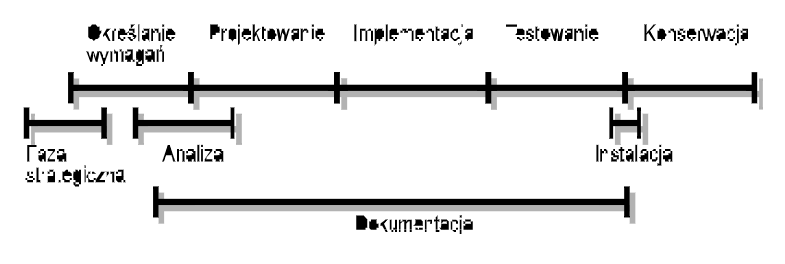
\includegraphics[width=0.9\textwidth]{model_kaskadowy}
      \caption{Model kaskadowy}
      \label{fig:cascade}
    \end{figure}
    Każda z faz cechuje się innym zestawem czynności jakie należy wykonać. 
    W fazie strategicznej głównie zachodzi rozmowa z klientem, opracowywany jest cel przedsięwzięcia, zakres, ogólne wymagania i analiza rozwiązań.
    Określony również zostaje wstępny harmonogram działań nad projektem.\\
    Faza określenia wymagań cechuje się, jak sama nazwa wskazuje, określeniem wymagań. Cele podane w fazie poprzedniej są zamieniane na faktyczne wymagania 
    jakie musi posiadać oprogramowanie. Wymagania dzielimy odpowiednio na funkcjonalne i niefunkcjonalne. 
    Wymagania funkcjonalne to takie, które opisują funkcję lub czynności wykonywane przez system. 
    Z koleji niefunkcjonalne opisują ograniczenia, przy zachowaniu których system powinien realizować swoje funkcję.\\
    W fazie analizy odpowiada się na pytanie: jak system ma działać? 
    W odpowiedzi na to pytanie otrzymujemy model systemu, opisujący jak postawione wymagania zostaną zrealizowane, nie wchodząc w szczegóły implementacyjne.\\
    W fazie projektowania ponownie odpowiada się na pytanie, tym razem jak system ma być zaimplementowany. W wyniku czego powstaje projekt sposobu implementacji.\\
    Kolejno przchodzi się do fazy implementacji, jest to moment, w którym wszystkie czynności związane z projektowaniem zostają zakończone i wcielone w faktyczny program.\\
    Po fazie implementacji następuje faza testowania. 
    W tej fazie następuje sprawdzenie systemu, czy jest zgodny z postawionymi wymaganiami, 
    oraz czy nie posiada jakichś błędów mogących doprowadzić do nieporządanego działania lub błędów z samym wykonywaniu się oprogramowania.\\
    W kolejnej fazie, czyli fazie instalacji, następuje przekazanie systemu użytkownikowi, pod koniec czego staje się on właścicielem systemu. 
    W skład tej fazy wchodzi dodatkowo: szkolenie użytkowników i administratorów, instalacja sprzętu i przeniesienie oprogramowania czy wypełenienie baz danych.\\
    Na samym końcu cyklu życia oprogramowania, znajduje się część przeznaczona na konserwację programu. 
    W tej fazie poprawiana jest jakość produktu, dostosowanie oprogramowania do zmian zachodzących w środowisku pracy oraz usuwanie wcześniej niewykrytych błędów.\\
    Warto również wspomnieć o fazie dokumentacji, jak widać na obrazku \ref{fig:cascade}, jest on wykonywany równolegle z praktycznie wszystkimi pozostałymi czynnościami. 
    Tworzona jest dokumentacja, w której znajdują się takie elementy jak: podręcznik użytkownika, opis instalacji czy podręcznik administratora. 
    Dokumentacja jest integralną częścią projektu i nie powinna być pomijana lub traktowana bez należytej uwagi.
  }
}

\section{Narzędzia i technologie wybrane do realizacji projektu}
{
  \subsection{Node.js}
  {
    "Node.JS jest jest wieloplatformowym oprogramowaniem o otwartym kodzie, 
    które pozwala deweloperom na tworzenie wszelkiego rodzaju oprogramowania w języku JavaScript pracującym po stronie serwera. 
    Jest to środowisko uruchomieniowe, które działa poza przeglądarką, współpracujące bezpośrednio z systemem operacyjnym. 
    W ten sposób środowisko Node udostępnia swoim aplikacjom API systemu operacyjnego, w tym dostęp do systemu plików, bibliotek systemowych czy uruchomionych procesów, 
    w tym serwerów HTTP."\cite{mozilla-node} Wartym wspomnienia jest fakt, że jest oparty na silniku JavaScript Chrome V8.\\ 
    Zalety jakie niesie ze sobą Node:
    \begin{itemize}
      \item wysoka wydajność, został zaprojektowany tak aby optymalizować wydajność i skalowalność aplikacji webowych
      \item pracując nad kodem po stronie klienta jak i po stronie serwera, poruszamy się w tym samym języku programowania
      \item dostęp do manadżera pakietów np. Yarn czy NPM, dzięki niemu uzyskuje się dostęp do setek tysięcy przeróżnych pakietów.
      \item jest przenośny. Można korzystać z niego zarówno na systemie macOS, Linux, jak również Windows.
      \item Dostęp do ogromnego community, gotowego służyć pomocą.
    \end{itemize}
    Node.JS jest bardzo uniwersalnym narzędziem, nie służy jedynie do tworzenia serwerów back endowych dla stron internetowych. Można za jego pomocą tworzyć 
    zwykłe aplikacje, aplikacje z dziedziny IoT(Internet of Things), posiada nawet pakiety do uczenia maszynowego. Za pomocą Node jesteśmy w stanie 
    wykonać przeróżne rzeczy ogranicza jedynie znajomość JavaScript oraz własna wyobraźnia. \\
    \begin{figure}[H]
      \centering
      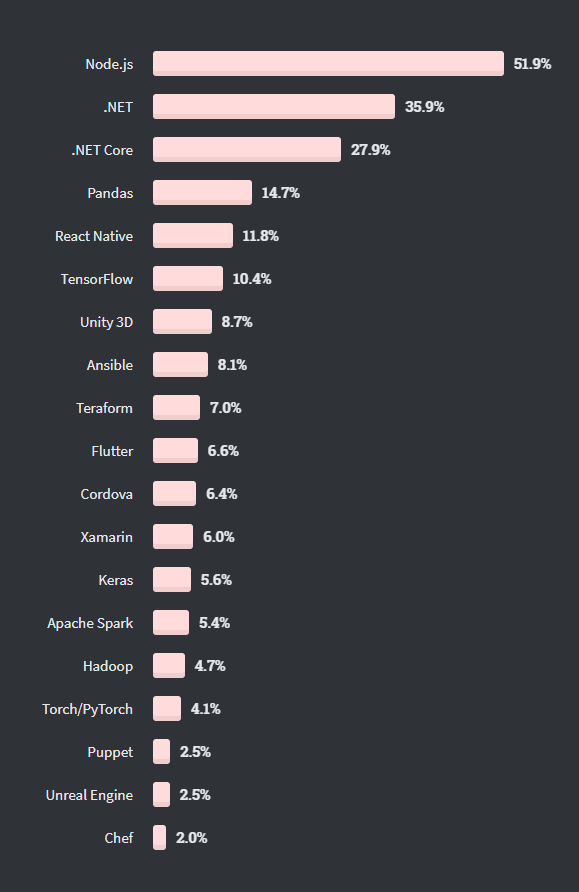
\includegraphics[width=0.9\textwidth]{most_popular_frameworks.PNG}
      \caption{Najpopularniejsze frameworki i biblioteki według ankiety Stack Overflow\cite{stack-survey}}
      \label{fig:backend}
    \end{figure}
    Jak zostało zaprezentowane na obrazku \ref{fig:backend}, Node.JS cieszy się ogromną popularnością. Uzyskał 51.9\% na 33 913 ankietowanych, 
    tę grupę stanowili jedynie profesjonalni developerzy.
    \begin{figure}[H]
      \centering
      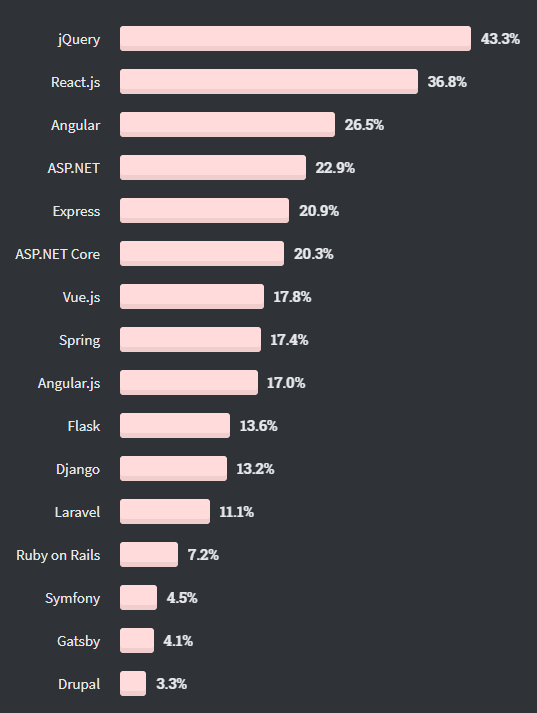
\includegraphics[width=0.9\textwidth]{most_popular_web_frameworks.PNG}
      \caption{Najpopularniejsze webowe frameworki według ankiety Stack Overflow\cite{stack-survey}}
      \label{fig:web-frameworks}
    \end{figure}
    Dodatkowo Express, czyli framework do Node.JS, za pomocą, którego został stworzony cały back end projektu, znajduje się na drugim miejscu w rankingu popularności 
    wśród frameworków back endowych, osiągnął popularność na poziomie 20.9\%. Wyprzedza takie frameworki jak: Java Spring, Flask, Django, Laravel czy Ruby on Rails, 
    jedynie ASP.NET plasuje się wyżej w rankingu. 
  }
  \subsection{React.js}
  {
    "React A JavaScript library for building user interfaces."\cite{react} Tłumacząc na polski, React jest biblioteką do tworzenia interfejsów użytkownika. 
    React jest oparty na komponentach, każdy komponent może posiadać własny stan i nim zarządzać, korzystając z komponentów można tworzyć bardzo złożone UI. 
    Sporym plusem Reacta jest fakt, że raz poznany umożliwia również tworzenie aplikacji mobilnych przy wykorzystaniu React Native. Co dodatkowo wyróżnia React 
    jest własna składnia, zbliżona do XML-a, czyli JSX. Jest to wymieszanie HTML-a i JavaScriptu, możemy dzięki niemu bez najmniejszych przeszkód umieszczać 
    tagi znane z HTML-a, w kodzie JavaScriptowym, przy tworzeniu komponentów. Dodatkowo własne komponenty, również podczas tworzenia struktury dokumenty, mają 
    składnię taką jak HTML. \\
    Kolejnym wyjątkowym aspektem Reacta jest Virtual DOM. Jest to koncept programistyczny gdzie wirtualna reprezentacja UI jest 
    przetrzymywana w pamięci i synchronizowana z prawdziwym DOM-em. 
    Umożliwia to podawanie UI w jakim stanie ma się znajdować i jakie komponenty mają być wyrenderowane, również upewnia się, że faktyczny DOM odowiada temu stanowi. 
    Ściagą to z programisty konieczność stworzenia samemu takich elementów jak: obsługę wydarzeń np. kliknięcie przycisku, manualne aktualizowanie DOM-u oraz manipulację atrybutami.
    \begin{figure}[H]
      \centering
      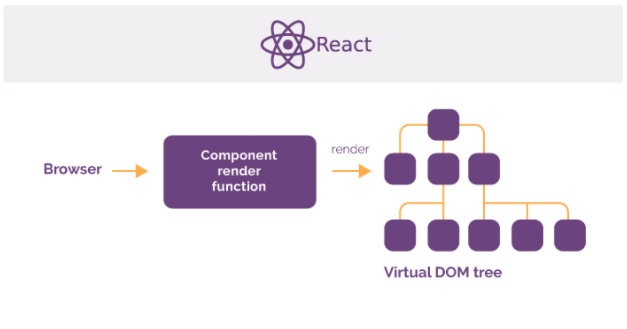
\includegraphics[width=0.9\textwidth]{how_react_works.PNG}
      \caption{Skrótowa prezentacja działania Reacta}
      \label{fig:how-react-works}
    \end{figure}
    Konkurencje dla Reacta stanowi Angular i Vue, jednakże to React króluje zarówno jeśli chodzi o popularność, pobrania, gwiazdki na GitHubie, liczbe pakietów, które są zależne od Reacta. 
    Niekwestionowym mistrzem jest również w kategoriach GitHub "Used by", tematach tworzonych na GitHubie.\cite{frontend-popularity} Dodatkowym atutem przemawiającym za Reactem jest 
    ilość pracy na rynku. Jak zostało zaprezentowane na obrazku poniżej, ponownie React króluje i w tej kategorii. 
    \begin{figure}[H]
      \centering
      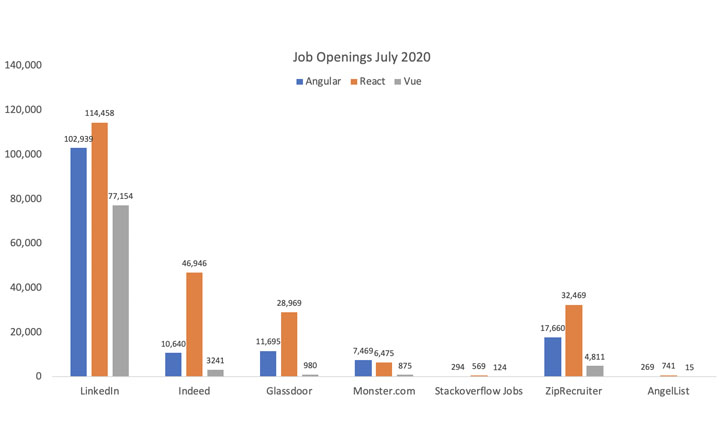
\includegraphics[width=0.9\textwidth]{frontend_jobs.jpg}
      \caption{Zapotrzebowanie na rynku, na specjalistów z danego frameworku.\cite{accenture}}
      \label{fig:frontend-jobs}
    \end{figure}
  }
  \subsection{TypeScript}
  {
    Czym jest TypeScript? W skrócie jest to JavaScript rozszerzający go o statyczne definicje typów, takie jak np. string, number czy boolean. 
    Został stworzony przez firmę Microsoft, przy wsparciu Google.
    Pisząc w TypeScripcie nie trzeba używać typów, inteferfejsów, typów generycznych czy też innych elementów udostępnianych. 
    Można pisać zwykły JavaScript i pomimo, że zostaną wyświetlone błędy informujące o nieokreślonym typie, cały kod wykona się mimo wszystko.
    Każdy kod napisany w JavaScripcie będzie w pełni funkcjonalnym kodem TypeScriptowym.
    Jednakże pisząc w TypeScripcie przeglądarka nie rozumie tego języka, zna tylko i wyłącznie JavaScript, dlatego kod musi być kompilowany przy pomocy 
    TypeScriptowego kompilatora lub Babela.\cite{typescript-docs} 
    Dodatkowo sprawia to, że napisany kod będzie działał na dowolnym urządzeniu i przeglądarce, o ile te wspierają JavaScript.\\
    Dlaczego programiści decydują się na TypeScript?\\
    Wynika to przede wszystkim z obecności typów, pisząc w JavaScripcie należałoby pisać dodatkowe linijki kodu tylko i wyłącznie sprawdzające np. czy 
    dane otrzymane przez serwer są odpowiednich typów, TypeScript robi wszystko za programiste. 
    Błędy związane z typami należą do najczęściej popełnianych wśród programistów JavaScript, szczególnie w projektach o większej skali bardzo łatwo o takie błędy.
    Typować można nie tylko zmienne, ale też funkcje, zarówne argumenty jakie przyjmuje oraz typ zwracany.\\
    TypeScript to nie tylko typy, posiada liczne dodatkowe funkcje, których JavaScript nie posiada. Są to chociażby wcześniej wspomnieniane interfejsy, 
    można deklarować własne typy, typy generyczne oraz typy wyliczeniowe - enumy. Inną niedostępna funkcją jest chociażby przeciążanie funkcji. 
    Wyglądem nie przypomina to kodu znanego z języków programowania typu Java czy C++, lecz spełnia dokładnie takie samo zadanie jak w tamtych językach.
  }
  \subsection{Najistotniejsze wykorzystane biblioteki}
  {
    W tej sekcji mogłoby znaleźć się ogromna ilość przeróżnych bibliotek, które są używane w projekcie. Create-React-App(służy do generowania projektów Reactowych), 
    sam w sobie pobiera kilkadziesiąt bibliotek. Tutaj jednak znajdą się tylko biblioteki, który zostały dodane na potrzeby projektu i warto o nich wspomnieć, a są to:
    \begin{itemize}
      \item Express
      \item Mongoose
      \item Stripe
      \item Nodemailer
      \item QRCode
      \item Material UI
      \item React Redux
      \item jsonwebtoken
      \item bcrypt
    \end{itemize}
    Pierwsza z nich czyli Express, jest minimalistycznym, elastycznym frameworkiem do Node.js. Dostarcza takie mechanizmy jak\cite{express}:
    \begin{itemize}
      \item Tworzenie funkcji obsługujących żądania metod HTTP i routing.
      \item Integrację z różnymi silnikami do generowania widowków, opartych na szablonach stron.
      \item Konfiguracja podstawowych ustawień aplikacji webowych np. port.
      \item Dodatkowe przetwarzanie żądań warstwy pośredniej(Middleware).
    \end{itemize}
    Sam w sobie Express jest minimalistyczny i nie posiada wielu istotnych funkcji. Dopiero zewnętrzne biblioteki umożliwiają takie aspekty jak: logowanie użytkowników,
    walidacja danych, zarządzanie ciasteczkami czy też parsowanie.\\

    Drugi z nich czyli Mongoose, służy do porozumiewania się z bazą danych MongoDB. Umożliwia w prosty sposób tworzenie modeli danych, walidację, przeszukiwanie bazy danych 
    oraz zapisywanie zmian w bazie. Lecz sam w sobie jest zdefiniowany jako narzędzie do modelowanie danych.\\

    Kolejną spośród wymienionych bibliotek jest Stripe. Stripe jest biblioteką do obsługi płatności internetowych, poprzez podanie danych karty kradytowej lub debetowej, 
    wysyłane jest zapytanie do API, które tworzy płatność, pobiera odpowiednią kwotę z konta i informuje o powodzeniu lub niepowodzeniu tranzakcji.\\

    Nodemailer jest prostym modułem dla aplikacji opartych na Node.js umożliwiającym i znacznie upraszczającym wysyłanie maili. Jest on o tyle niezbędny, że każdy bilet wysyłany jest na maila, 
    jedynie zalogowani użytkownicy mają wgląd do histori tranzakcji i mogą podejrzeć kod QR z poziomu aplikacji. Użytkownicy goście nie mają innego dostępu do biletów, jedynie 
    przychodzą one na maila.\\

    QRCode jest biblioteką do generowania kodów QR. Jest to technologia bardzo obecnie popularna i wygodna, praktycznie każdy obecny smartfon posiada czytnik kodów QR.\\

    Material UI jest jedną z najpopularniejszych bibliotek komponentów. Służy do tworzenia interfejsów użytkownika, bazując na gotowych komponentach, dodatkowo znacznie 
    usprawniając tworzenie responsywnych interfejsów.\\

    React Redux jest to biblioteka do Reacta, udostępniająca przetrzymywanie globalnego stanu aplikacji i dostępu do niego z każdego jej poziomu. Jest to o tyle przydatne 
    narzędzie, że bez jego wykorzytsania developer byłby zmuszony do przekazywania danych między komponentami w bardzo nieelegancki i toporny sposób. Redux umożliwia 
    manipulację i dostęp do globalnego stanu z dowolnego komponentu.\\

    Jsonwebtoken jest biblioteką do tworzenia JWT, służący przede wszystkim do autoryzacji użytkownika, szczególnie przydatne jest to przy logowaniu. Szerzej o JWT 
    przedstawione zostanie w jednej z kolejnych podsekcji.\\

    Bcrypt - prosta biblioteka do hashowania hasła użytkownika, wykorzystywana przy rejestracji nowych użytkwoników.
  }
  \subsection{MongoDB}
  {
    MongoDB jest typem nierelacyjnej bazy danych, posiada strukturę zbliżoną do JSON-a, czyli klucz-wartość. Oznacza to, że każdy dokument może mieć inną strukturę, 
    zupełnie inaczej niż jest to w relacyjnych bazach. MongoDB charakteryzuje się wysokim bezpieczeństwem, dużą skalowalnością i łatwością obsługi. 
    Świadczyć o tym może fakt, że z usług tej bazy danych korzystają takie firmy jak Google, Adobe czy ebay. \\
    MySQL vs MongoDB\\
    MySQL jest popularną, darmową i open-source relacyjną bazą danych stworzoną przez firmę Oracle. Jak w 
  }
  \subsection{JWT - JSON Web Token}
  {
    Jest otwartym standardem (RFC 7519), który definiuje kompaktową i samowystarczalną możliwość, bezpiecznej transmisji danych w formacie JSON\cite{jwt}. 
    Informacje przekazywane za pomocą JWT są weryfikowalne i można im ufać, ponieważ są podpisywane cyfrowo. 
    JWT można podpisać za pomocą algorytmu HMAC przy wykorzystaniu sekretu lub pary klucza publicznego i prywatnego przy wykorzystaniu algorytmów RSA lub ECDSA. 
    Sekret jest tajnym hasłem przechowywanym przez serwer do podpisywania i autoryzacji tokenów.
    Najczęstszym powodem wykorzystania JWT jest auotryzacja użytkownika, czy to przy logowaniu, czy też 
    przy sprawdzaniu dostępu do np. jakiegoś url w aplikacji. Innym popularnym zastosowaniem jest wymiana informacji.\\
    JSON Web Token składa się z następujących elementów: nagłówka (Header), payloadu oraz podpisu, oddzielonych od siebie kropkami. 
    Przeważnie struktura JWT wygląda następująco: xxxxx.yyyyy.zzzzz\\
    Nagłówek przeważnie składa się z dwóch części: typu wygenerowanego tokena oraz algorytmu, jakim został podpisany.\\
    Payload jest odpowiedzialny za przetrzymywanie danych zawartych w tokenie.\\
    Zarówno nagłówek, jak i payload są kodowane za pomocą Base64-URL do stworzenia odpowiednio pierwszej i drugiej części JWT.\\
    Do stworzenia podpisu należy wziąć zakodowany nagłówek i payload, spreyzować algorytm szyfrujący oraz prywatny klucz lub sekret i podpisać to.
    Przykładowo przy wykorzystaniu algorytmu HMAC SHA256, podpis zostanie stworzony w następujący sposób:\\
    \begin{figure}[H]
      \centering
      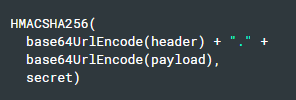
\includegraphics[width=0.9\textwidth]{JWT_signature.PNG}
      \caption{Sposób tworzenia podpisu JWT przy wykorzystaniu algorytmu HMAC SHA256.}
      \label{fig:jwt_signature}
    \end{figure}
    Wynikiem takiej operacji są trzy ciągi znaków Base64-URL, oddzielonych od siebie kropkami.\\
    JWT w tworzonej aplikacji wykorzystywane jest przy rejestracji, logowaniu oraz dostępu do niektórych ścieżek. 
    Rejestracja przebiega następująco:
    \begin{enumerate}
      \item Użytkownik podaje dane niezbędne do rejestracji.
      \item Użytkownik zatwierdza podane dane.
      \item Wysyłane jest zapytanie do serwera, gdzie tworzony jest token, hashowane jest hasło i tworzony nowy wpis w bazie danych.
    \end{enumerate}
    Dzięki temu po zalogowaniu użytkownik ma dostęp do inaczej niedostępnej sekcji, czyli histori zamówień, gdzie można zaleźć wszystkie posiadane bilety wraz z ich kodami QR.
  }
}

\section{Proces tworzenia aplikacji}
{

}

\section{Podsumowanie}
{

}

\section{Możliwości dalszego rozwoju aplikacji}
{

}

\section{Bibliografia}
{
  \printbibliography
}

\section{Spis rysunków}
{
  \listoffigures
}

\section{Spis tabel}
{
  \listoftables
}

\end{sloppypar}
\end{document}
